%!TEX root = ../main.tex

\section{\texorpdfstring{$\CP$}{CP} violation in \texorpdfstring{$\bToccbard$}{bToccbard} decays}
\label{sec:cpviolation:btoccbard}

The decay \BdToDD can be described with the Feynman diagrams in
\cref{fig:cpviolation:feynmandiagrams_bdtodd}.
\begin{figure}[htb]
\centering
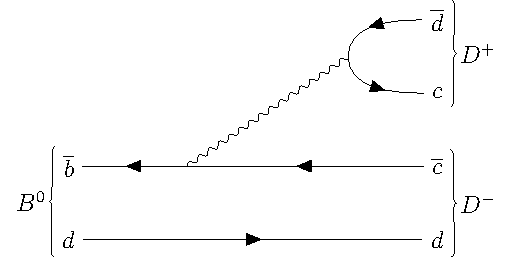
\includegraphics[width=0.48\textwidth]{03-CPViolation/tikz/pdf/BdToDD_Tree.pdf}
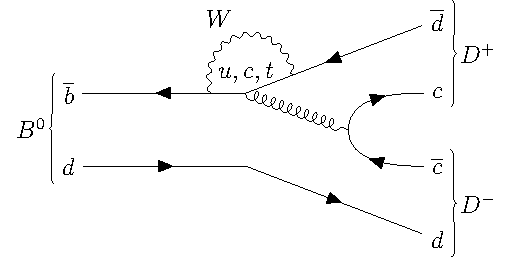
\includegraphics[width=0.48\textwidth]{03-CPViolation/tikz/pdf/BdToDD_Penguin.pdf}
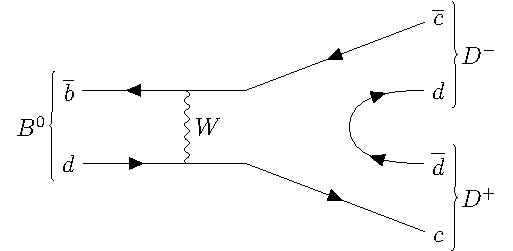
\includegraphics[width=0.48\textwidth]{03-CPViolation/tikz/pdf/BdToDD_Exchange.pdf}
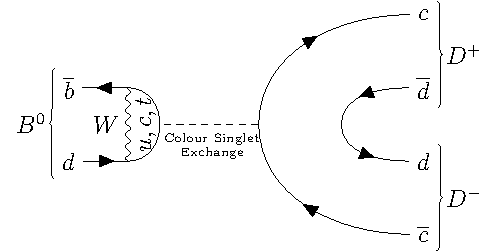
\includegraphics[width=0.48\textwidth]{03-CPViolation/tikz/pdf/BdToDD_Annihilation.pdf}
\caption{Main Feynman diagrams contributing to \BdToDD decays. Apart from the
tree diagram (top left), a penguin diagram (top right), an exchange diagram
(bottom left) and a penguin annihilation diagram (bottom right) are shown.}
\label{fig:cpviolation:feynmandiagrams_bdtodd}
\end{figure}
The tree diagram ($T$) proceeds via a \bToccbard quark transition, which is
CKM suppressed. The contributions from the other diagrams, especially the
penguin diagrams ($P^{(q)}$ with $q = \uquark$, \cquark and \tquark quarks in the
loop), but also exchange ($E$) and penguin annihilation diagrams
($P\!A^{(q)}$), need to be taken into account as well, because they can carry
different weak phases and are not Cabibbo-suppressed. Thus, the decay
amplitude is given by~\cite{Fleischer1999,Fleischer2007,Bel:2015wha}
\begin{align}
\begin{split}
	A(\BdToDD) &= \Vcbs\Vcd T + \Vtbs\Vtd P^{(t)} + \Vcbs\Vcd P^{(c)} + \Vubs\Vud P^{(u)}\\
			   &+ \Vcbs\Vcd E + \Vcbs\Vtd P\!A^{(t)} + \Vcbs\Vcd P\!A^{(c)} + \Vubs\Vud P\!A^{(u)}\,.
\end{split}
\end{align}
Using the CKM unitarity condition
\begin{align}
	\Vtbs\Vtd + \Vcbs\Vcd + \Vubs\Vud = 0 \quad\Leftrightarrow\quad \Vtbs\Vtd = - \Vcbs\Vcd - \Vubs\Vud
\end{align}
the decay amplitude can be written as
\begin{align}
\begin{split}
	A(\BdToDD) &= \Vcbs\Vcd \left(T + E + \left\{P^{(c)} + P\!A^{(c)}\right\} - \left\{P^{(t)} + P\!A^{(t)}\right\}\right)\\
			   &+ \Vubs\Vud \left(\left\{P^{(u)} + P\!A^{(u)}\right\} - \left\{P^{(t)} + P\!A^{(t)}\right\}\right)\,.
\end{split}
\end{align}
With the definition
\begin{align}
	\mathcal{A} \equiv \left[T + E + \left\{P^{(c)} + P\!A^{(c)}\right\} - \left\{P^{(t)} + P\!A^{(t)}\right\}\right]\,,
\end{align}
this can be further simplified to
\begin{align}
	A(\BdToDD) = \Vcbs\Vcd \mathcal{A}\left[1 + \frac{\Vubs\Vud}{\Vcbs\Vcd} \frac{\left\{P^{(u)} + P\!A^{(u)}\right\} - \left\{P^{(t)} + P\!A^{(t)}\right\}}{\mathcal{A}}\right]\,.
\end{align}
Applying the Wolfenstein parametrisation and plugging in the definitions of the
side length $R_b$ (see \cref{eq:cpviolation:Rb}) and of the angle $\gamma$ of
the unitarity triangle (see \cref{eq:cpviolation:angles})
\begin{align}
\begin{split}
	\frac{\Vubs\Vud}{\Vcbs\Vcd} &= -\left(1 - \frac{\lambda^2}2\right)\frac 1\lambda \left|\frac \Vub\Vcb\right| \text{arg}\left(\frac{\Vubs\Vud}{\Vcbs\Vcd}\right)\\
	&= -R_b e^{-i\gamma}\,,
\end{split}
\end{align}
the decay amplitude becomes
\begin{align}
	A(\BdToDD) = \Vcbs\Vcd \mathcal{A}[1 - ae^{i\theta}e^{-i\gamma}]\,,
\end{align}
with
\begin{align}
	ae^{i\theta} \equiv R_b\left[\frac{\{P^{(u)} + P\!A^{(u)}\} - \{P^{(t)} + P\!A^{(t)}\}}{T + E + \left\{P^{(c)} + P\!A^{(c)}\right\} - \left\{P^{(t)} + P\!A^{(t)}\right\}}\right]\,.
\end{align}
While $\gamma$ is a \CP-violating weak phase, $a$ and $\theta$ are hadronic
\CP-conserving parameters. Therefore, the corresponding \Bzb decay amplitude
is
\begin{align}
	A(\BdbToDD) = \Vcb\Vcds \mathcal{A}[1 - ae^{i\theta}e^{i\gamma}]\,.
\end{align}
The parameter describing \CP violation in the interference can be written as
\begin{align}
\begin{split}
	\lambda_{\Dp\Dm} &= \frac{\Vtbs\Vtd}{\Vtb\Vtds}\frac{\Vcb\Vcds}{\Vcbs\Vcd}\frac{1-ae^{i\theta}e^{i\gamma}}{1-ae^{i\theta}e^{-i\gamma}}\,,\\
					 &= e^{-i2\beta}\frac{1-ae^{i\theta}e^{i\gamma}}{1-ae^{i\theta}e^{-i\gamma}}\,,
\end{split}
\end{align}
using the ratio of the mixing coefficients from
\cref{eq:cpviolation:qp_simplified} and the definition of the unitarity
triangle $\beta$ from \cref{eq:cpviolation:angles}. Different than for
\BdToJPsiKS (cf.~\cref{eq:lambda_JPsiKS}) the \CP eigenvalue is $\eta_{\CP} =
\num{+1}$, since no angular momenta are involved in the decay \BdToDD. The
hadronic parameters cannot be calculated reliably within
QCD~\cite{Bel:2015wha}. Thus, they must be determined through a measurement of
the \CP observables, which can be expressed via
\begin{align}
	\CDD &= \frac{1 - |\lambda|^2}{1 + |\lambda|^2} = \frac{2a\sin\theta\sin\gamma}{1 - 2a\cos\theta\cos\gamma + a^2}\,,\\
	\SDD &= \frac{2\,\mathcal{I}m\,\lambda}{1 + |\lambda|^2} = -\frac{\sin\phid - 2a \cos\theta\sin(\phid + \gamma) + a^2\sin(\phid + 2\gamma)}{1 - 2a\cos\theta\cos\gamma + a^2}\,.
\end{align}
Due to interferences between tree and penguin contributions \CDD might differ
from zero. The term \SDD, which is caused by interference between the direct
decay and the decay after mixing, gives access to the mixing phase \phid.
However, different than in the case of \BdToJPsiKS decays only an effective
phase
\begin{align}
	\phideff = \phid + \Delta\phid
\end{align}
with
\begin{align}
	\sin\phideff = -\frac{\SDD}{\sqrt{1 - \CDD^2}}
\end{align}
can be measured in \BdToDD. The phase shift $\Delta\phid$ is given by
\begin{align}
	\tan\Delta\phid = \frac{a^2\sin2\gamma - 2a\cos\theta\sin\gamma}{1 - 2a\cos\theta\cos\gamma + a^2\cos2\gamma}\,.
\end{align}

The decay channel \BsToDsDs is related to \BdToDD via U-spin symmetry. It is
governed by a \bToccbars transition and gives access to \phis. The
measurement is as well polluted by hadronic penguin effects. Here, the phase
shift is given by
\begin{align}
	\tan\Delta\phis = \frac{\epsilon^2a'^2\sin2\gamma + 2\epsilon a'\cos\theta'\sin\gamma}{1 + 2\epsilon a'\cos\theta'\cos\gamma + \epsilon^2a'^2\cos2\gamma}\,.
\end{align}
The factor
\begin{align}
	\epsilon \equiv \frac{\lambda^2}{1 - \lambda^2} = \num{0.0536\pm0.0003}
\end{align}
reduces the impact of the phase shift. However, in the concept of U-spin symmetry
\begin{align}
	ae^{i\theta} = a'e^{i\theta'}\,.
\end{align}
Thus, with a measurement of \CP violation in \BdToDD decays, where the phase
shift is not suppressed by $\epsilon$, the hadronic parameters $a$ and
$\theta$ can be determined precisely, and then transferred to the measurement
of \CP violation in \BsToDsDs decays.

Further decay modes from the family of \BToDDbar decays are \BdToDstD and
\BdToDstDst, which also enable a determination of \phideff, but introduce
further complications. For \BdToDstD the final state is not a \CP eigenstate
as it can be distinguished by the charge of the \Dstarpm meson. Thus, four \CP
observables are needed to describe \CP violation. Furthermore, from an
experimentalist's point of view the final state is not symmetrical in terms of
the charges of pions and kaons and thus a detection asymmetry has to be taken
into account. In the measurement of \CP violation using \BdToDstDst decays,
like for \BsToJPsiPhi decays, an angular-dependent analysis is required.
